% !TEX program = pdflatex
% !TEX encoding = UTF-8 Unicode

\documentclass{beamer}
\usepackage[utf8]{inputenc}
\usepackage[T1]{fontenc}
\usepackage{lmodern}
\usepackage{amsmath,amssymb}
\usepackage{graphicx}
\usepackage{booktabs}
\usepackage{hyperref}
\usepackage{tikz}
\usetikzlibrary{arrows.meta, positioning, shapes.geometric, fit, calc}

\usetheme{Madrid}
\usecolortheme{default}

% Custom colors for better visuals
\definecolor{darkblue}{RGB}{0,51,102}
\definecolor{lightblue}{RGB}{173,216,230}
\definecolor{darkgreen}{RGB}{0,102,51}
\setbeamercolor{structure}{fg=darkblue}

%------------------------------------------------------------
% Title page configuration
%------------------------------------------------------------
\title[BDH Searchless Chess]{BDH-GPU for Searchless Chess}
\subtitle{Training a Post-Transformer Architecture\\on Chess Position Evaluation}

\author{Antoni Czapski}

\institute[]{
  Project: Deep Learning\\
  Proposal Presentation
}

\date{March 10, 2026}

%------------------------------------------------------------
% Table of contents at each section
%------------------------------------------------------------
\AtBeginSection[]
{
  \begin{frame}
    \frametitle{Outline}
    \tableofcontents[currentsection]
  \end{frame}
}

%------------------------------------------------------------
\begin{document}

%------------------------------------------------------------
% Title
%------------------------------------------------------------
\frame{\titlepage}

%------------------------------------------------------------
% Table of Contents
%------------------------------------------------------------
\begin{frame}
\frametitle{Outline}
\tableofcontents
\end{frame}

%==============================================================================
\section{Problem Definition}
%==============================================================================

%------------------------------------------------------------
\begin{frame}
\frametitle{Searchless Chess: The Problem}

\begin{columns}
\column{0.55\textwidth}
\textbf{Task:} Predict chess position quality from a static board state --- no tree search allowed.

\vspace{0.5em}
\begin{itemize}
    \item \textbf{Input:} Board position (FEN notation)
    \item \textbf{Output:} Score $\in [-1, 1]$\\(normalized Stockfish centipawn)
    \item \textbf{Formulation:} Supervised regression
\end{itemize}

\vspace{0.5em}
No minimax. No alpha-beta. No MCTS.\\
\alert{Pure neural intuition.}

\column{0.45\textwidth}
\begin{block}{Prior Art}
\footnotesize
\begin{tabular}{lrc}
\toprule
\textbf{Model} & \textbf{Params} & \textbf{ELO} \\
\midrule
DeepMind & 270M & 2895 \\
ViT-Med$^*$ & 9.5M & 1960 \\
ViT-Small$^*$ & 2.6M & 1817 \\
ResNet-XL$^*$ & 24.7M & 1719 \\
\bottomrule
\end{tabular}

\vspace{0.3em}
$^*$Grzyb, 2025
\end{block}

\vspace{0.3em}
\footnotesize Key insight: ViTs achieve \alert{10$\times$ better} parameter efficiency than ResNets for chess.
\end{columns}

\end{frame}

%------------------------------------------------------------
\begin{frame}
\frametitle{My Angle: Why BDH?}

\begin{columns}
\column{0.55\textwidth}
\textbf{Research question:}\\
Can a \alert{post-transformer} architecture (BDH-GPU) match or beat ViT on searchless chess?

\vspace{1em}
\textbf{Why BDH suits chess:}
\begin{enumerate}
    \item \textbf{Relational state} --- piece interactions (pins, forks, batteries) stored as neuron-pair weights
    \item \textbf{Iterative reasoning} --- shared-weight layers applied $K$ times, like ``thinking longer''
    \item \textbf{Sparse activations} --- only relevant motifs fire, matching chess pattern recognition
\end{enumerate}

\column{0.45\textwidth}
\begin{block}{BDH in One Sentence}
A recurrent linear-attention model with \alert{Hebbian fast-state updates} and \alert{weight-tied layers}.
\end{block}

\vspace{0.5em}
\begin{alertblock}{Novelty}
No prior work has applied BDH to chess or any combinatorial game domain.
\end{alertblock}
\end{columns}

\end{frame}

%==============================================================================
\section{Dataset}
%==============================================================================

%------------------------------------------------------------
\begin{frame}
\frametitle{Dataset: Lichess-Stockfish-Normalized}

\begin{columns}
\column{0.55\textwidth}
\textbf{Source:} HuggingFace (CC BY 4.0)\\
{\footnotesize\url{huggingface.co/datasets/mateuszgrzyb/lichess-stockfish-normalized}}

\vspace{0.5em}
\begin{table}
\centering
\footnotesize
\begin{tabular}{lr}
\toprule
\textbf{Property} & \textbf{Value} \\
\midrule
Total positions & 316M \\
Format & Parquet (10 shards) \\
Deduplication & FEN-based \\
Key columns & \texttt{fen, cp, depth} \\
Original source & Lichess.org \\
\bottomrule
\end{tabular}
\end{table}

\vspace{0.3em}
\textbf{I use:} $\sim$50--100M subset\\(compute-constrained to 100h A100)

\column{0.45\textwidth}
\begin{block}{Input Encoding}
FEN $\rightarrow$ \texttt{8$\times$8$\times$12} tensor

\vspace{0.3em}
\footnotesize
\begin{itemize}
    \item 64 squares $\times$ 12 channels
    \item Binary piece-type occupancy
    \item Always-white perspective\\(board mirrored for black)
\end{itemize}
\end{block}

\vspace{0.5em}
\begin{block}{Data Split}
\begin{tabular}{lr}
Train & 90\% \\
Validation & 5\% \\
Test & 5\% \\
Seed & \texttt{2001} \\
\end{tabular}
\end{block}
\end{columns}

\end{frame}

%------------------------------------------------------------
\begin{frame}
\frametitle{Data Pipeline}

\begin{center}
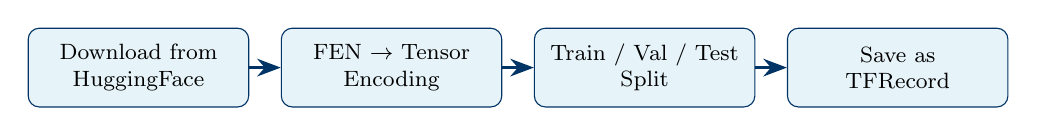
\begin{tikzpicture}[
    node distance=0.8cm and 0.4cm,
    box/.style={rectangle, draw=darkblue, fill=lightblue!30, rounded corners,
                minimum height=1cm, minimum width=2.8cm, align=center, font=\footnotesize},
    arrow/.style={-{Stealth[length=3mm]}, thick, darkblue}
]

\node[box] (dl) {Download from\\HuggingFace};
\node[box, right=of dl] (enc) {FEN $\rightarrow$ Tensor\\Encoding};
\node[box, right=of enc] (split) {Train / Val / Test\\Split};
\node[box, right=of split] (tfr) {Save as\\TFRecord};

\draw[arrow] (dl) -- (enc);
\draw[arrow] (enc) -- (split);
\draw[arrow] (split) -- (tfr);

\end{tikzpicture}
\end{center}

\vspace{0.5em}
\begin{columns}
\column{0.5\textwidth}
\begin{block}{Reusable Components}
\begin{itemize}
    \item \texttt{fen\_to\_tensor()} --- proven encoding from existing repo
    \item \texttt{mate\_to\_cp()} --- mate $\rightarrow$ centipawn conversion
    \item TFRecord streaming for memory efficiency
\end{itemize}
\end{block}

\column{0.5\textwidth}
\begin{block}{Engineering Decisions}
\begin{itemize}
    \item \textbf{Deterministic} splits (seeded shuffle)
    \item \textbf{Config-driven} --- all paths \& params in YAML
    \item \textbf{Scripted} download --- \texttt{datasets} library
    \item \textbf{No raw data} in Git
\end{itemize}
\end{block}
\end{columns}

\end{frame}

%==============================================================================
\section{Evaluation Metric}
%==============================================================================

%------------------------------------------------------------
\begin{frame}
\frametitle{Evaluation Strategy}

\begin{columns}
\column{0.5\textwidth}
\textbf{Training Metric:}
$$\mathcal{L} = \text{MSE}(\hat{y}, y) = \frac{1}{N}\sum_{i=1}^{N}(\hat{y}_i - y_i)^2$$

\vspace{0.3em}
\textbf{Monitoring:} MAE for interpretability

\vspace{1em}
\textbf{Gold Standard: ELO Estimation}
\begin{enumerate}
    \item Solve 1,200 Lichess puzzles\\(12 tiers, 100 per tier)
    \item Accuracy per tier
    \item Linear regression fit
    \item \alert{ELO = rating at 50\% accuracy}
\end{enumerate}

\column{0.5\textwidth}
\begin{block}{Why Puzzles Are Valid}
\footnotesize
Searchless models evaluate only the \textbf{immediate position} (depth = 1).

\vspace{0.3em}
$\Rightarrow$ Puzzle difficulty $\equiv$ pattern recognition complexity

\vspace{0.3em}
$\Rightarrow$ 50\% threshold $\approx$ human-equivalent strength at that rating
\end{block}

\vspace{0.5em}
\begin{block}{Puzzle Dataset}
\footnotesize
Already available:\\
\texttt{data/puzzles/test\_puzzles.feather}
\begin{itemize}
    \item Ratings: 399 -- 3213 ELO
    \item Proven methodology (Grzyb, 2025)
\end{itemize}
\end{block}
\end{columns}

\end{frame}

%==============================================================================
\section{Architecture}
%==============================================================================

%------------------------------------------------------------
\begin{frame}
\frametitle{BDH-GPU Architecture}

\begin{center}
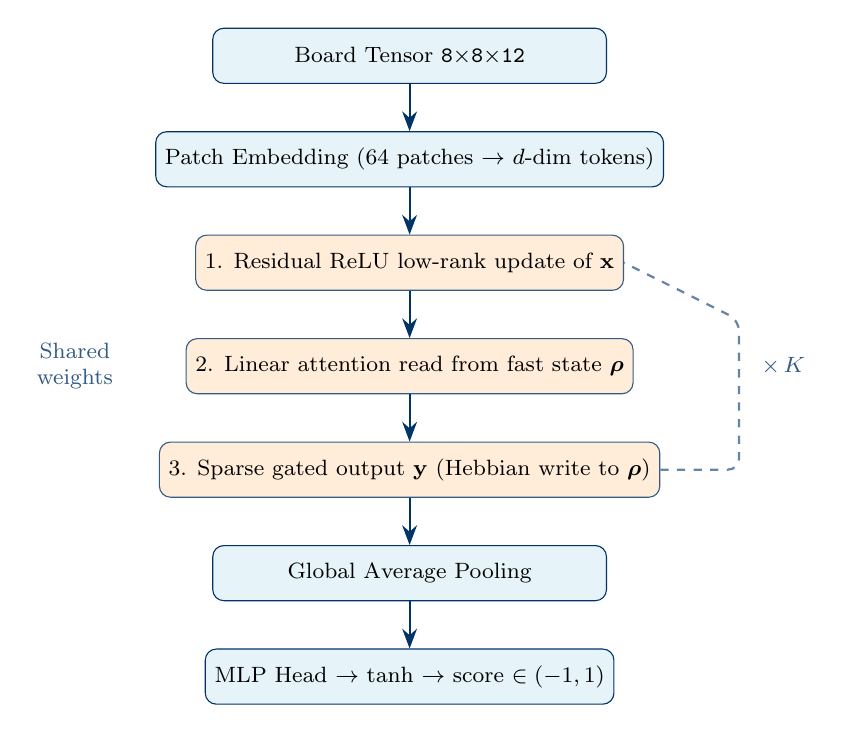
\begin{tikzpicture}[
    node distance=0.6cm,
    box/.style={rectangle, draw=darkblue, fill=lightblue!30, rounded corners,
                minimum height=0.7cm, minimum width=5cm, align=center, font=\footnotesize},
    recbox/.style={rectangle, draw=darkblue!80, fill=orange!15, rounded corners,
                minimum height=0.7cm, minimum width=5cm, align=center, font=\footnotesize},
    arrow/.style={-{Stealth[length=2.5mm]}, thick, darkblue},
    loopline/.style={thick, darkblue!60, dashed}
]

\node[box] (input) {Board Tensor \texttt{8$\times$8$\times$12}};
\node[box, below=of input] (embed) {Patch Embedding (64 patches $\rightarrow$ $d$-dim tokens)};
\node[recbox, below=of embed] (step1) {1. Residual ReLU low-rank update of $\mathbf{x}$};
\node[recbox, below=of step1] (step2) {2. Linear attention read from fast state $\boldsymbol{\rho}$};
\node[recbox, below=of step2] (step3) {3. Sparse gated output $\mathbf{y}$ (Hebbian write to $\boldsymbol{\rho}$)};
\node[box, below=of step3] (pool) {Global Average Pooling};
\node[box, below=of pool] (head) {MLP Head $\rightarrow$ $\tanh$ $\rightarrow$ score $\in (-1, 1)$};

\draw[arrow] (input) -- (embed);
\draw[arrow] (embed) -- (step1);
\draw[arrow] (step1) -- (step2);
\draw[arrow] (step2) -- (step3);
\draw[arrow] (step3) -- (pool);
\draw[arrow] (pool) -- (head);

% Recurrence loop
\node[right=1.5cm of step2, font=\footnotesize\bfseries, text=darkblue!80] (klabel) {$\times\,K$};
\draw[loopline, rounded corners] (step3.east) -- ++(1.0,0) -- ++(0, 1.9) -- (step1.east);

% Brace for shared weights
\node[left=0.8cm of step2, font=\footnotesize, text=darkblue!80, align=center] {Shared\\weights};

\end{tikzpicture}
\end{center}

\end{frame}

%------------------------------------------------------------
\begin{frame}
\frametitle{Model Variants \& Baselines}

\begin{columns}
\column{0.55\textwidth}
\textbf{BDH-GPU Variants:}
\begin{table}
\centering
\footnotesize
\begin{tabular}{lccc}
\toprule
\textbf{Variant} & $n$ & $K$ & \textbf{Params} \\
\midrule
BDH-Tiny & 4096 & 4 & $\sim$1.6M \\
BDH-Small & 8192 & 8 & $\sim$6.3M \\
BDH-Medium & 16384 & 12 & $\sim$12.6M \\
\bottomrule
\end{tabular}
\end{table}

\vspace{0.5em}
$n$ = neuron dimension, $d = 256$ (rank),\\
$K$ = recurrent depth (shared weights)

\vspace{0.5em}
\textbf{Key Experiment:}\\
Depth ablation --- $K \in \{4, 8, 12\}$\\
\emph{Does more ``thinking'' help?}

\column{0.45\textwidth}
\textbf{Baselines for Comparison:}
\begin{table}
\centering
\footnotesize
\begin{tabular}{lcc}
\toprule
\textbf{Model} & \textbf{Params} & \textbf{ELO$^*$} \\
\midrule
MLP & $\sim$2M & $\sim$900 \\
ViT-Small & 2.6M & 1817 \\
\bottomrule
\end{tabular}

\vspace{0.3em}
{\tiny $^*$Expected / known from prior work}
\end{table}

\vspace{0.5em}
\begin{block}{Comparison Strategy}
\footnotesize
\begin{itemize}
    \item \textbf{Param-matched:} BDH-Tiny vs ViT-Small ($\sim$2.6M)
    \item \textbf{Scale:} BDH-Small/Medium
    \item \textbf{Ablation:} depth $K$ effect
\end{itemize}
\end{block}
\end{columns}

\end{frame}

%==============================================================================
\section{Engineering Plan}
%==============================================================================

%------------------------------------------------------------
\begin{frame}
\frametitle{Repository Structure}

\begin{columns}
\column{0.5\textwidth}
\begin{table}
\centering
\footnotesize
\begin{tabular}{ll}
\toprule
\textbf{Directory} & \textbf{Purpose} \\
\midrule
\texttt{.github/workflows/} & CI/CD pipeline \\
\texttt{configs/} & YAML experiment configs \\
\texttt{src/models/} & BDH, ViT, ResNet, CNN \\
\texttt{src/training/} & Unified training loop \\
\texttt{src/evaluation/} & Puzzle-based ELO eval \\
\texttt{src/data\_preparation/} & FEN encoding pipeline \\
\texttt{tests/} & pytest test suite \\
\texttt{scripts/} & Entry points \\
\texttt{notebooks/} & EDA \& analysis \\
\bottomrule
\end{tabular}
\end{table}

\column{0.5\textwidth}
\begin{block}{New Files (my contribution)}
\footnotesize
\begin{itemize}
    \item \texttt{src/models/\alert{bdh.py}} --- BDH-GPU implementation
    \item \texttt{src/training/\alert{trainer.py}} --- unified config-driven training
    \item \texttt{src/evaluation/\alert{puzzle\_evaluator.py}} --- ELO estimation
    \item \texttt{tests/\alert{test\_bdh\_model.py}} --- forward pass \& shape tests
    \item \texttt{tests/\alert{test\_training\_smoke.py}} --- 1-batch smoke test
\end{itemize}
\end{block}
\end{columns}

\end{frame}

%------------------------------------------------------------
\begin{frame}[fragile]
\frametitle{DevOps Toolchain}

\begin{columns}
\column{0.5\textwidth}
\begin{block}{Environment: \texttt{uv}}
\footnotesize
\begin{verbatim}
uv sync
uv run python scripts/training/train.py \
  --config configs/train_bdh_small.yaml
\end{verbatim}
\end{block}

\vspace{0.5em}
\begin{block}{CI/CD (GitHub Actions)}
\footnotesize
\begin{itemize}
    \item \texttt{ruff check} --- linting
    \item \texttt{ruff format --check} --- formatting
    \item \texttt{pytest tests/ -v} --- all tests
    \item Triggered on push \& PR to \texttt{main}
\end{itemize}
\end{block}

\column{0.5\textwidth}
\begin{block}{Testing (\texttt{pytest})}
\footnotesize
\begin{itemize}
    \item Data loading \& encoding
    \item BDH forward pass \& output shape
    \item Loss computation sanity check
    \item 1-batch training smoke test
    \item Evaluation pipeline test
\end{itemize}
\end{block}

\vspace{0.5em}
\begin{block}{Bonus Targets}
\footnotesize
\begin{itemize}
    \item Docker container
    \item Streamlit demo
    \item Inference benchmarking
    \item W\&B Sweeps
\end{itemize}
\end{block}
\end{columns}

\end{frame}

%------------------------------------------------------------
\begin{frame}[fragile]
\frametitle{Reproducibility \& Experiment Tracking}

\begin{columns}
\column{0.5\textwidth}
\textbf{Reproducibility Guarantees:}
\begin{table}
\centering
\footnotesize
\begin{tabular}{ll}
\toprule
\textbf{Requirement} & \textbf{Implementation} \\
\midrule
Random seeds & YAML $\rightarrow$ \texttt{tf}, \texttt{np}, \texttt{random} \\
Fixed splits & Seeded shuffle, saved to JSON \\
Config-driven & 1 YAML per experiment \\
Best model & \texttt{ModelCheckpoint} \\
Pinned deps & \texttt{uv.lock} \\
\bottomrule
\end{tabular}
\end{table}

\vspace{0.5em}
\textbf{Unified Entry Point:}\\
\footnotesize One script, any architecture:
\normalsize
{\footnotesize
\begin{verbatim}
uv run python scripts/training/train.py \
  --config configs/train_bdh_small.yaml
\end{verbatim}
}

\column{0.5\textwidth}
\textbf{Weights \& Biases Integration:}
\begin{itemize}
    \item All hyperparams logged automatically
    \item Training curves (loss, MAE)
    \item ELO estimates per experiment
    \item Model artifacts saved
\end{itemize}

\vspace{0.5em}
\begin{block}{Planned Experiments ($\geq$7)}
\footnotesize
\begin{enumerate}
    \item MLP baseline
    \item ViT-Small baseline
    \item BDH-Tiny ($K$=4)
    \item BDH-Small ($K$=8)
    \item BDH-Small depth ablation
    \item BDH-Medium ($K$=12)
    \item BDH + adaptive depth
\end{enumerate}
\end{block}
\end{columns}

\end{frame}

%==============================================================================
\section{Timeline, Risks \& Compute}
%==============================================================================

%------------------------------------------------------------
\begin{frame}
\frametitle{Compute Budget (100h A100)}

\begin{table}
\centering
\footnotesize
\begin{tabular}{lccl}
\toprule
\textbf{Task} & \textbf{Hours} & \textbf{Cumulative} & \textbf{Phase} \\
\midrule
Data pipeline + encoding & 2h & 2h & Infrastructure \\
MLP baseline & 2h & 4h & Baselines \\
ViT-Small baseline & 5h & 9h & Baselines \\
\midrule
BDH-Tiny (fast iteration) & 5h & 14h & BDH Development \\
BDH-Small (main model) & 20h & 34h & BDH Development \\
Depth ablation ($K$=4,8,12) & 15h & 49h & Ablations \\
\midrule
BDH-Medium (scale-up) & 40h & 89h & Advanced \\
Evaluation + misc & 5h & 94h & Evaluation \\
\alert{Buffer} & \alert{6h} & \alert{100h} & Safety \\
\bottomrule
\end{tabular}
\end{table}

\vspace{0.3em}
\begin{center}
\footnotesize
\textit{BDH-Medium is expendable --- if behind schedule, reallocate to more ablations.}
\end{center}

\end{frame}

%------------------------------------------------------------
\begin{frame}
\frametitle{Meeting Roadmap}

\begin{table}
\centering
\footnotesize
\begin{tabular}{clll}
\toprule
\textbf{\#} & \textbf{Meeting} & \textbf{Deliverable} & \textbf{Engineering Focus} \\
\midrule
3 & \alert{Proposal} & \alert{This presentation} & --- \\
4 & Repo \& CI & Public repo, CI green & \texttt{uv}, \texttt{ruff}, \texttt{pytest} \\
5 & EDA + Baseline & Notebooks, MLP/ViT & Data pipeline tests \\
6 & Reproducible & Config training, W\&B & Seeds, checkpoints \\
7 & First BDH & BDH-Tiny/Small results & W\&B $\geq$3 experiments \\
8 & Improvements & Tuning, depth ablation & Before/after comparison \\
9 & Error Analysis & Failure by puzzle tier & Overfit/underfit analysis \\
10 & Advanced & BDH-Medium, ablations & W\&B $\geq$7 experiments \\
11 & Final Review & Clean repo, README & CI green, all tests pass \\
12 & Presentation & 15--20 min final & Full results + conclusions \\
\bottomrule
\end{tabular}
\end{table}

\end{frame}

%------------------------------------------------------------
\begin{frame}
\frametitle{Risks \& Mitigations}

\begin{columns}
\column{0.5\textwidth}
\begin{alertblock}{High Risk}
\textbf{BDH underperforms ViT}\\
\footnotesize \textit{Mitigation:} Still valid as architecture comparison study. Strong baselines ensure meaningful contribution regardless.
\end{alertblock}

\vspace{0.3em}
\begin{alertblock}{High Risk}
\textbf{No reference implementation}\\
\footnotesize \textit{Mitigation:} Start with BDH-Tiny, extensive unit tests, verify gradient flow early. \textit{(Also: bonus for engineering quality.)}
\end{alertblock}

\column{0.5\textwidth}
\begin{block}{Medium Risk}
\textbf{Compute overrun}\\
\footnotesize \textit{Mitigation:} Strict hour tracking. BDH-Medium is expendable.
\end{block}

\vspace{0.3em}
\begin{block}{Low Risk}
\textbf{Data pipeline issues}\\
\footnotesize \textit{Mitigation:} Reuse proven pipeline. HuggingFace \texttt{datasets} handles downloading.
\end{block}

\vspace{0.3em}
\begin{exampleblock}{Fallback Strategy}
\footnotesize If BDH fails to converge $\rightarrow$ simplify (remove Hebbian updates, reduce to linear attention) $\rightarrow$ project becomes ``Lessons Learned'' with strong engineering.
\end{exampleblock}
\end{columns}

\end{frame}

%==============================================================================
\section{Summary}
%==============================================================================

%------------------------------------------------------------
\begin{frame}
\frametitle{Summary}

\begin{enumerate}
    \item \textbf{Problem:} Searchless chess --- predict position quality without search\\
    {\footnotesize Supervised regression: FEN $\rightarrow$ score $\in [-1, 1]$}
    
    \vspace{0.5em}
    \item \textbf{Dataset:} 316M positions (Lichess-Stockfish-Normalized, HuggingFace)\\
    {\footnotesize Proven to produce 1960 ELO models}
    
    \vspace{0.5em}
    \item \textbf{Architecture:} BDH-GPU --- post-transformer with Hebbian state\\
    {\footnotesize 3 scales (1.6M--12.6M params), depth ablation $K \in \{4, 8, 12\}$}
    
    \vspace{0.5em}
    \item \textbf{Metric:} MSE (training) + ELO via 1200 puzzle benchmark\\
    {\footnotesize Direct comparison to ViT-Small (1817 ELO)}
    
    \vspace{0.5em}
    \item \textbf{Engineering:} \texttt{uv} + CI/CD + \texttt{ruff} + \texttt{pytest} + W\&B + YAML configs\\
    {\footnotesize Config-driven, reproducible, $\geq$7 tracked experiments}
\end{enumerate}

\vspace{0.5em}
\begin{center}
\large\alert{Compute: 100h on NVIDIA A100}
\end{center}

\end{frame}

%------------------------------------------------------------
\begin{frame}
\frametitle{Thank You!}

\begin{center}
\Large
\textbf{Questions?}

\vspace{2em}
\normalsize
\begin{tabular}{ll}
\textbf{Dataset:} & \footnotesize\url{huggingface.co/datasets/mateuszgrzyb/lichess-stockfish-normalized} \\[0.3em]
\textbf{Reference repo:} & \footnotesize\url{github.com/mateuszgrzyb-pl/searchless-chess} \\[0.3em]
\textbf{BDH paper:} & \footnotesize Available upon request \\
\end{tabular}

\vspace{2em}
\begin{block}{}
\centering
\footnotesize
Input: \texttt{8$\times$8$\times$12} board tensor
$\;\xrightarrow{\text{BDH-GPU ($K$ passes)}}\;$
Output: position score $\in (-1, 1)$
\end{block}
\end{center}

\end{frame}

%==============================================================================
% Backup slides
%==============================================================================

\appendix

\begin{frame}
\frametitle{Backup: BDH-GPU Core Equations}

\textbf{Trainable parameters:} $E, D_x, D_y \in \mathbb{R}^{n \times d}$\\
Total: $\approx (3 + o(1)) \cdot n \cdot d$

\vspace{1em}
\textbf{Per-layer recurrence (simplified):}

\begin{enumerate}
    \item \textbf{Update activations:}
    $\mathbf{x}_{l} \leftarrow \mathbf{x}_{l-1} + \text{ReLU}(D_x \cdot \mathbf{v})$
    
    \item \textbf{Read from fast state:}
    $\mathbf{a}_{l} = E \cdot \boldsymbol{\rho}_{l-1} \cdot \mathbf{x}_{l}$
    
    \item \textbf{Produce sparse output:}
    $\mathbf{y}_{l} = \text{SparseGate}(\mathbf{a}_{l})$
    
    \item \textbf{Hebbian state update:}
    $\boldsymbol{\rho}_{l} = \boldsymbol{\rho}_{l-1} + \mathbf{v}^*_{l} \cdot \mathbf{x}_{l}^T$
    \hfill where $\mathbf{v}^*_{l} = E^T \mathbf{y}_{l}$
\end{enumerate}

\vspace{0.5em}
\textbf{Key property:} Same weights at every layer $\rightarrow$ variable depth $K$ is free.

\end{frame}

\begin{frame}[fragile]
\frametitle{Backup: YAML Config Example}

{\footnotesize
\begin{verbatim}
experiment:
  name: "bdh-small-k8"
  seed: 2001
  wandb_project: "bdh-searchless-chess"

model:
  architecture: "bdh"
  n_neurons: 8192
  d_rank: 256
  k_depth: 8
  dropout: 0.1

training:
  epochs: 100
  learning_rate: 1e-4
  min_learning_rate: 1e-6
  weight_decay: 1e-4
  batch_size: 512
  scheduler: "cosine"
  mixed_precision: true

callbacks:
  early_stopping: {patience: 5, monitor: "val_loss"}
  wandb: {enabled: true}
\end{verbatim}
}

\end{frame}

\begin{frame}
\frametitle{Backup: ELO Estimation Method}

\begin{enumerate}
    \item \textbf{1,200 puzzles} across 12 difficulty tiers (399--3213 ELO)
    \item For each tier: $\text{accuracy} = \frac{\text{correct puzzles}}{100}$
    \item Fit linear regression: $\text{Rating} = f(\text{Accuracy})$
    \item \textbf{ELO estimate} = predicted rating at \alert{50\% accuracy}
\end{enumerate}

\vspace{1em}
\textbf{Example from prior work (Grzyb, 2025):}

\vspace{0.5em}
\begin{table}
\centering
\footnotesize
\begin{tabular}{lccc}
\toprule
\textbf{Model} & \textbf{Tier 4} (1000) & \textbf{Tier 6} (1500) & \textbf{Tier 8} (2000) \\
\midrule
CNN (1.18M) & 43\% & 22\% & 7\% \\
ViT-Small (2.6M) & 82\% & 68\% & 34\% \\
ViT-Medium (9.5M) & 88\% & 86\% & 45\% \\
\bottomrule
\end{tabular}
\end{table}

\end{frame}

\end{document}
